\documentclass{article}
\usepackage[utf8]{inputenc}
\usepackage{amsmath}
\usepackage{graphicx}
\usepackage{float}
\usepackage[font=scriptsize,labelfont=bf]{caption}

\title{COMP6245 : Lab 2 Report}
\author{Thanakorn Panyapiang(31446612)}
\date{}

\begin{document}
\maketitle

\section{Implementing the Perceptron algorithm}
Given the data which has the distribution like Figure 1a, using the Perceptron algorithm to train a linear classifier gives a decision boundary as shown in Figure 1b. It can be noticed that the accuracy improves as numbers of iteration increase which can be observed from Figure 1c.
\begin{center}
\begin{tabular}{ccc}
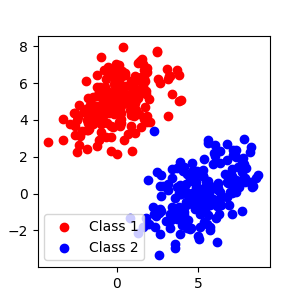
\includegraphics[scale=0.3]{scatter_sample1} &
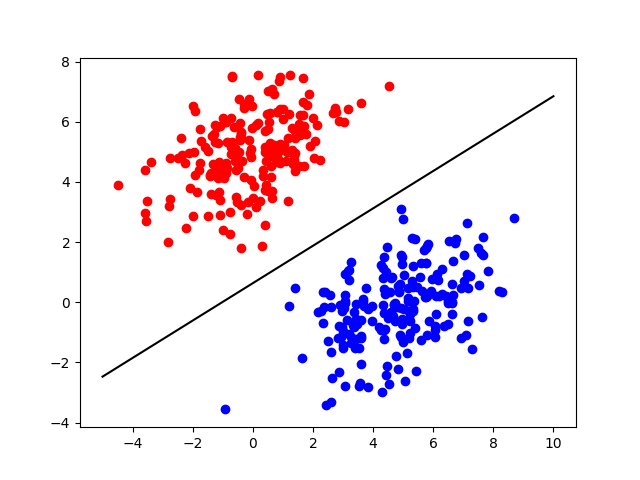
\includegraphics[scale=0.2]{sample1_decision_doundary} &
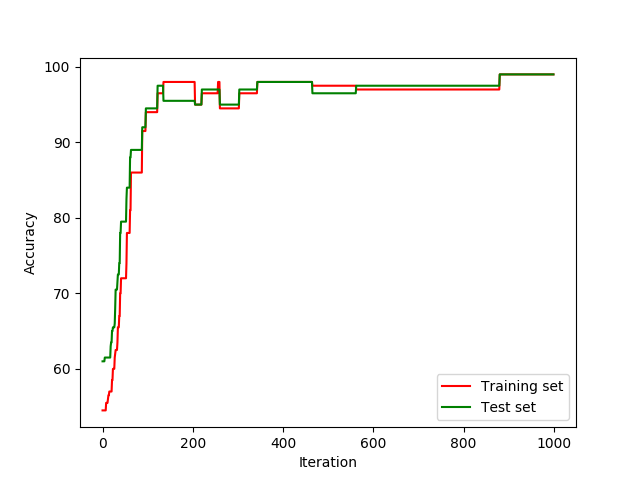
\includegraphics[scale=0.2]{learning_curve_sample1} \\
\scriptsize a & \scriptsize b & \scriptsize c\\
\end{tabular}
\captionof{figure}{}
\end{center}

However, the algorithm fails to train a decent linear classifier for the sample which has the distribution like Figure 2a as can be seen from the decision boundary and the accuracy in Figure 2b. and 2c. respectively.
\begin{center}
\begin{tabular}{ccc}
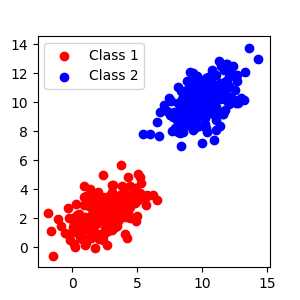
\includegraphics[scale=0.3]{scatter_sample2} &
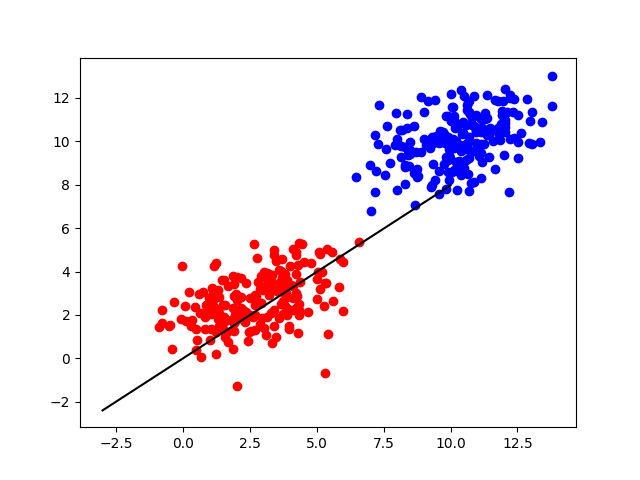
\includegraphics[scale=0.2]{sample2_decision_doundary} &
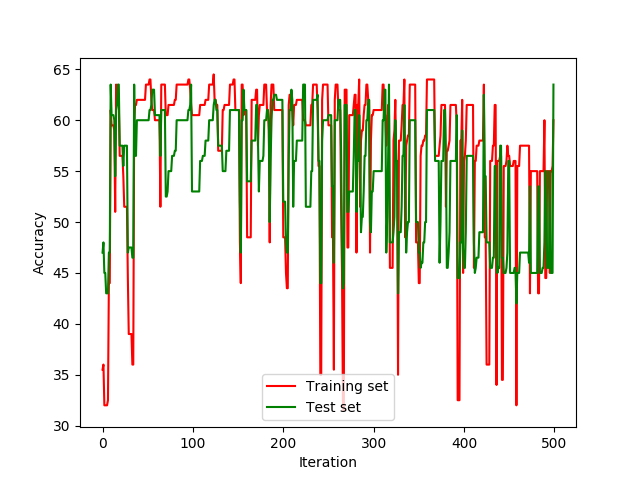
\includegraphics[scale=0.2]{learning_curve_sample2} \\
\scriptsize a & \scriptsize b & \scriptsize c\\
\end{tabular}
\captionof{figure}{}
\end{center}

The cause of this issue is the algorithm tries to find the decision boundary that passes the origin, but unlike the first dataset, there is no line which passes the origin that can split two classes in this dataset.\\
\indent To fix this issue, the algorithm needs to be modified so that the decision boundary doesn't have to pass the origin. This can be done by adding a bias feature to the dataset which will allow the algorithm to shift the decision boundary. The result after adding a bias feature is shown in Figure 3.

\begin{center}
\begin{tabular}{cc}
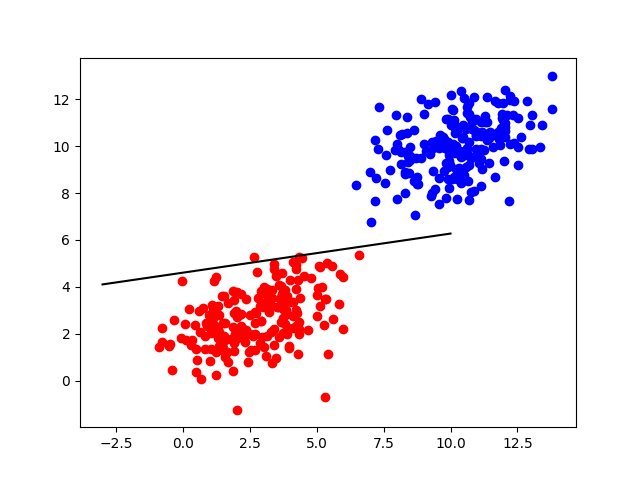
\includegraphics[scale=0.3]{sample2_decision_doundary_bias} &
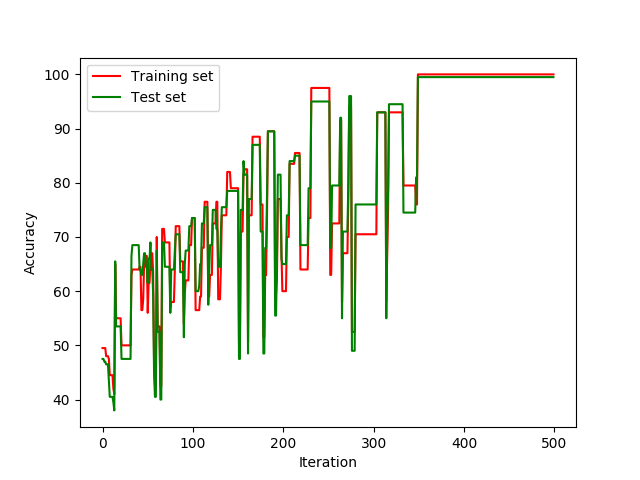
\includegraphics[scale=0.3]{learning_curve_sample2_bias} \\
\scriptsize a & \scriptsize b\\
\end{tabular}
\captionof{figure}{}
\end{center}

\section{Testing with a benchmark dataset}
The benchmark dataset which is used to test the algorithm is the Iris dataset. From the scatter plot in Figure 4a and 4b, it can be noticed that the data can be separated using only two attributes. 
\begin{center}
\begin{tabular}{cc}
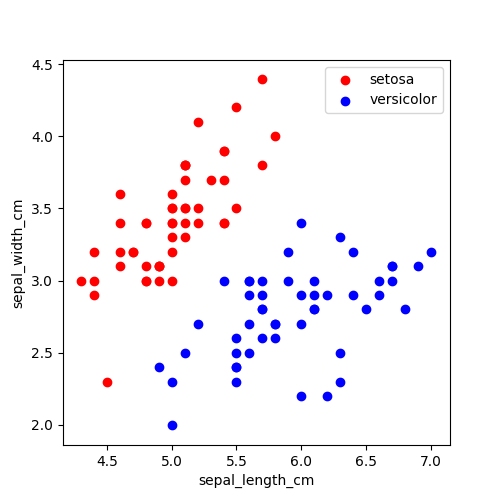
\includegraphics[scale=0.3]{sepal_compare} &
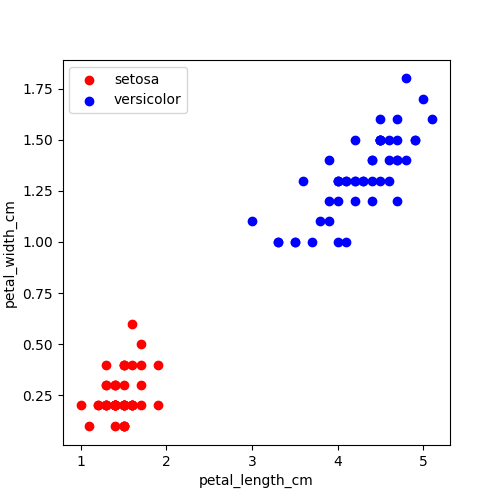
\includegraphics[scale=0.3]{petal_compare} \\
\scriptsize a & \scriptsize b\\
\end{tabular}
\captionof{figure}{}
\end{center}

Training a linear classifier for the Iris dataset using the Perceptron algorithm gives the result as illustrated in Figure 5. The model trained from sepal width and sepal length(Figure 5a) give 100 percent accuracy while the classifier trained using petal width and petal length(Figure 5b) has 99 percent accuracy.
\begin{center}
\begin{tabular}{cc}
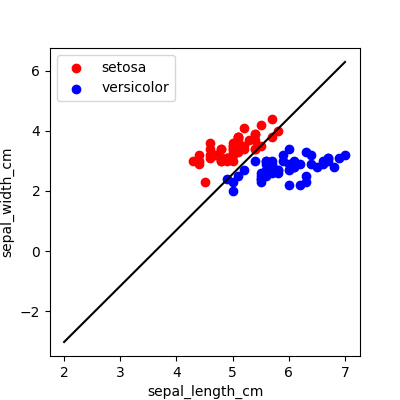
\includegraphics[scale=0.35]{sepal_decision} &
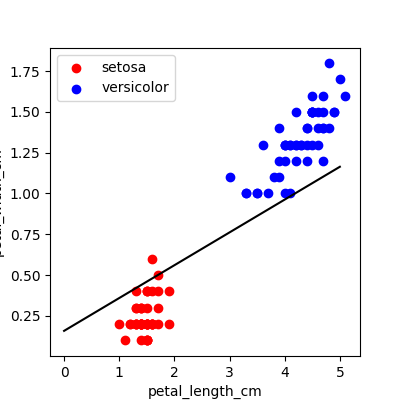
\includegraphics[scale=0.35]{petal_decision} \\
\scriptsize a & \scriptsize b\\
\end{tabular}
\end{center}

\end{document}